% !TEX encoding = UTF-8 Unicode
\documentclass{article}
\usepackage{amsmath}
\usepackage{mathtools}
\usepackage{graphicx, color}
\graphicspath{{figs/}}
\usepackage{natbib}
\usepackage{hyperref}

%----------------------------------
%\topmargin      -1.5cm   % read Lamport p.163
%\oddsidemargin  -0.04cm  % read Lamport p.163
%\evensidemargin -0.04cm  % same as oddsidemargin but for left-hand pages
%\textwidth      16.59cm
%\textheight     22.94cm

\topmargin      -1.5cm   % read Lamport p.163
\oddsidemargin  -0.5cm  % read Lamport p.163
\evensidemargin -0.5cm  % same as oddsidemargin but for left-hand pages
\textwidth      16cm
\textheight     22.94cm

\parskip         7.2pt   % sets spacing between paragraphs
\parindent         3mm   % sets leading space for paragraphs

\setcounter{topnumber}{2}
\setcounter{bottomnumber}{2}
\setcounter{totalnumber}{4}
\renewcommand{\topfraction}{0.85}
\renewcommand{\bottomfraction}{0.85}
\renewcommand{\textfraction}{0.15}
\renewcommand{\floatpagefraction}{0.7}

\bibpunct{(}{)}{;}{a}{}{,} 

%-------------------------------------

\title{Bayesian Inference for  Covariance Matrix}
\author{Ignacio Alvarez}
\date{ Spring 2014 }

\begin{document}
\maketitle 
\thispagestyle{empty}

\begin{abstract}
Covariance matrix estimation is a common and usually difficult task in statistics. We present a comparative study for some covariance matrix prior choices on the context of Bayesian hierarchical linear models. In Bayesian analysis an inverse Wishart distribution is the natural choice for a covariance matrix prior because its conjugacy on normal model and simplicity, is usually available in Bayesian statistical software. However inverse Wishart distribution presents some undesirable properties from a modeling point of view. It can be too restrictive because assume the same amount of prior information about every variance parameters and, more important, it shows a prior relationship between the variances and correlations.

Two alternatives distributions has been proposed. The scaled inverse Wishart distribution, which give more flexibility on the variance priors conserving the conjugacy property but does not eliminate the prior relationship between variances and correlations. Secondly, it is possible to fit separate priors for individual correlations and standard deviations. This strategy eliminates any prior relationship within the covariance matrix parameters, but it is not conjugate and therefore computationally slow. 

The objective of this study is to understand the impact of these prior choices on the covariance matrix posterior.

We applied a hierarchical model with the different covariance priors using a forest bird monitoring program data provided for the Natural Resources Research Institute as an example. Data consist in the yearly bird count for 73 species on three National Forest from 1995 to 2013.
\end{abstract}
\newpage 

\linespread{1.5}

\tableofcontents
\thispagestyle{empty}

\newpage 

\section{Introduction} 

The estimation of a covariance matrix is a important issue on statistics, appears on multivariate problems but most commonly on the hierarchical model context. The inclusion of random effects in a linear model within Bayesian framework may lead to modeling the covariance matrix for those effects. Also regression models with varying coefficients across groups is one of the most common situation where a prior for a covariance matrix is needed. 

Bayesian estimation of covariance matrix is a difficult problem, mainly because the standard approaches of conjugacy or non-informativeness present problems.  The natural conjugate prior for the multivariate normal distribution is the inverse Wishart distribution. Conjugacy property has made of this choice the most commonly used approach for covariance matrix. However this model present some problems due to its lack of flexibility and dependency among correlation and variances.  On the other hand, Jeffrey covariance prior may lead to improper posterior distributions when it is used in hierarchical models. 

There are many alternative ways to construct priors for the covariance matrices that have been proposed,  however \cite{visualize} states that 
 \textit{''but even fewer analytical results are known for these families, making it even more challenging to understand precisely the properties of such distributions. Consequently, our analytical understanding of these distributions falls short of providing us a full understanding of the inverse-Wishart distribution'' }

Broadly we can organize these alternatives in a few categories. A first strategy is to decompose the covariance matrix into more components, secondly it is possible to use the inverse Wishart prior but putting priors on its parameters to give more flexibility. Finally a third way to approach this problem is to model a transformation of the covariance matrix. 
 
\begin{description}
\item[Decomposition] There are several ways to decompose a covariance matrix.  \cite{yang1994} use a spectral decomposition for the covariance matrix and develop a reference prior for the component matrices. 

\cite{barnard2000} separate the covariance matrix in correlations and variances, with log-normal prior on the standard deviations and a independent prior for the correlation matrix, which is based on the inverse Wishart distribution transformed into a correlation matrix. This kind of decomposition is appealing from an applied modeling perspective, since seem to be easier incorporate prior information for individual variances or correlations than fot a whole matrix. However, it turns out that this later prior for correlation is hard to use and present some computations problems, \cite{SIW2008} propose a scaled inverse Wishart approach based on the separation strategy which is recommended in \cite{gelmanhill}. \cite{lewandowski2009generating} develop an alternative prior for correlation matrices that could be used in combination with this separation strategy. 

\item[Hierarchical] The inverse Wishart distribution has two parameters, a matrix location parameter and scalar degrees of freedom parameter.  Building a hierarchical structure is appealing allows data dependent shrinkage of the estimated covariance matrix. Letting $W \sim IW(\nu,\Lambda)$ is the inverse Wishart distribution, \cite{daniels1999} use flat priors for $\nu$ and the diagonal entries of $\Lambda$. Then, \cite{matilde} follow the same approach with a re-parametrization that ensure a proper posterior.  Recently,  \cite{huang2013simple} used only prior for the diagonals entries on $\Lambda$ with inverse gamma distribution. 

\item[Transformation] As imposing a prior for covariance matrix is hard, it may be better to model it implicitly. \cite{wong2003} propose a prior for the precision matrix, the inverse of covariance matrix, \cite{leonard1992} use a prior on the logarithm of the covariance matrix and \cite{smith2002} use a prior on the Cholesky factor for the precision matrix which and apply it to longitudinal data.
However, these approaches are somewhat computationally complicated and fairly complicated for interpretation. 
\end{description}

The objective of this study is to understand the impact of some prior choices on the covariance matrix posterior. We select some of the proposed prior models in the literature , with these options we first run a simulation study to assess the impact on posterior and we then apply each model  to a real data set consisting of bird counts on national forest in the Great Lakes. 

We use the standard conjugate model inverse Wishart prior, because is the most used model in practice. We also consider the separation strategy proposed by  \cite{barnard2000} and scaled inverse Wishart approach, among decomposition models these two are the more promising from an end user perspective because its interpretation (the former) or its applicability (the latter). Finally we consider the hierarchical approach proposed by \cite{huang2013simple}, this is the most recent proposal we found for this problem. 

The rest of this paper is organized as follows: next section described the statistical methods and the covariance prior distributions we use. Then we present a simulation study consisting in simulate from data from a multivariate normal model and make inference about the covariance matrix to compare the different priors. Finally to see if what we learned from simulated data is translated on a real data example we estimate the correlation among bird species counts using yearly bird count on Superior forest. 

\section{Statistical Models}

This section describes the statistical methods used in this paper, the main focus of this work will be on covariance matrix inference.  We compare the covariance matrix priors in the context of a  multivariate normal model. 

Whenever is needed, we will separate individual element in the matrix in order to better understand the effect of each prior distribution we consider. Let standard deviation for each group be denoted with $\sigma_i$ and the correlation among groups $i$ and $j$ denoted by $\rho_{ij}$. Then the diagonal entry will be $\Sigma_{ii} = \sigma_i^2$ and an entry outside the diagonal $\Sigma_{ij} = \sigma_i\sigma_j\rho_{ij}$. 


\subsection{Bayesian inference for covariance matrix within Multivariate Normal model }
 Let assume the $d$ dimensional vector $Y$ follows a multivariate normal distribution, $Y \sim N_d(0, \Sigma)$, we work with centered data, it is possible extend this to include a mean vector $\mu$ and perform a similar simulation exercise. However the focus here will be the inference about the covariance matrix and then we prefer not to deal with the mean estimation. A similar approach is took by  \cite{daniels1999}
and \cite{matilde} in their simulation exercises.
 
 Consider $n$ observations from $Y \sim N_d(0, \Sigma)$ distribution, the likelihood function can be written as follows : 
  \begin{eqnarray}
\nonumber  p(y\vert \mu,\Sigma) &\propto& |\Sigma|^{-n/2} e^{- \frac{1}{2} \sum_{i=1}^n y_i^{'} \Sigma^{-1} y_i  } \\
      &\propto& |\Sigma|^{-n/2} e^{- \frac{1}{2}  tr(\Sigma^{-1}S_0)  } 
 \label{like}
 \end{eqnarray} 
where $y_i$ represent the $i$th  observation from the vector $Y$, and $S_0=\sum_{i=1}^n y_i y_i ^{'}$.  
%In order to complete the model we need to specify priors on mean and variance parameters which are usually modeled as independents, i.e., $p(\mu,\Sigma) = p(\mu)p(\Sigma)$. Also it is common to use non informative priors on the mean such as a improper prior $p(\mu) \propto 1$ or very vague one like $N(0, M)$ for a big value of $M$. In all the models used in the paper we treat mean and covariance matrix as independent and use normal priors for the mean. 

Definite positive requirement for $\Sigma$ results in non trivial constrains for the matrix elements which makes difficult to set a prior distribution for it. This is the main reason of the existence of many different strategies to setting priors on covariance matrix.  We present here the two "default" options of non-informativeness and conjugacy with the main problems for these options. 

\subsubsection{ Conjugate prior}

Inverse Wishart (IW) is a distribution for the entire covariance matrix $\Sigma$, it has two parameters $\Lambda_0$ and $\nu_0$ that controls the center and scale of the distribution respectively, $\Lambda_0$ is a positive definite $d$ dimensional matrix and $\nu_0$ is a scalar value representing degrees of freedom.
 
\begin{eqnarray}
\nonumber \Sigma &\sim& IW(\nu_0,\Lambda_0) \\
p(\Sigma) &\propto& |\Sigma|^{-(\nu_0 + d +1)/2 } e^{-\frac{1}{2} tr( \Lambda_0 \Sigma^{-1}) }
\label{eq:wis}
\end{eqnarray}

In order to get a proper prior $\nu_0 > d$, this implies an inverse scale chi-square distribution for each variance $\sigma_i^2\sim inv\chi^2(\nu_0 - d + 1, \frac{\lambda_{ii}}{\nu_0-d+1} )$ where $\lambda_{ii}$ its a diagonal entry of $\Lambda$.  

Setting the parameters to get a non-informative priors is usually done by setting $\nu_0$, this is $\Lambda_0=I_d$ and $\nu_0=d+1$ where $I_d$ is an identity matrix of size $d$.  This parameter choice implies a marginal uniform distribution on all correlations.  At a multivariate level the prior mean is $E(\Sigma) = \Sigma_0= \frac{\Lambda_0}{\nu_0 - d - 1}$ 

The main advantages of $IW$ prior are the conjugacy on normal model and its simplicity, most of the software has this distribution have the option for an $IW$ distribution. Based on equations \ref{like} and \ref{eq:wis} we can derive the posterior distribution for $\Sigma$ as 

  \[
 p(\Sigma\vert y ) \propto |\Sigma|^{ -(\frac{n+\nu_0+d+1}{2} )} e{- \frac{1}{2} tr( (\Lambda_0+S_0)\Sigma^{-1} }
 \] 
 
implying $\Sigma \vert y \sim IW(n+\nu_0, \Lambda_0+S_0)$. Note $\frac{S_0}{n} = \frac{1}{n} \sum_{i=1}^n y_i y_i^{'} = \hat\Sigma_{mle}$ the MLE estimator of the covariance matrix, then we can write the posterior mean as follows 
\[  E(\Sigma\vert y) = \frac{\Lambda_0 + S_0}{n+\nu_0-d-1} = \frac{ (\nu - k-1)\Lambda_0 + n\hat\Sigma_{mle} } {n+\nu_0-d-1}  \] 

There are two main problems with the $IW$ prior. 
First, the uncertainty for all variance parameters (diagonal entries in the matrix) is controlled by the degree of freedom parameter, this could  be too restrictive since``implies the same amount of prior information about each of the variance parameters in the covariance matrix'' \cite{bda2003}. 

Secondly, this prior impose a dependency between $\rho_{ij}$ and $\sigma_i$, in particular higher values for the standard deviation $\sigma_i$ are associated with higher correlations, $\rho_{ij}$ close to 1 or -1.  This can be a major problem if we are specially interested on making inference for correlations, since $\rho_{ij}$ will be large for coefficients with higher variance independently of its relation,  we illustrate this aspect based on simulations. (\cite{visualize})

\subsubsection{Non-informative prior} 
The  Jeffrey prior for the model (\ref{like}) is $p(\Sigma)\propto |\Sigma| ^ {\frac{-(d+1)}{2} } $,  which its reduce to $p(\sigma) \propto \sigma^{-1}$  the usual conjugate prior for univariate model.  \cite{gelman2006prior} has showed this present problems for variance parameters within hierarchical models and \cite{SIW2008} extend this concerns to the multivariate case,  the main problem is that Jeffrey may lead to improper posterior within the context of linear models (\cite{SIW2008}).  

\subsection{Alternative priors for $\Sigma$}
We present the alternatives to IW prior we use in this work ordered in terms of it lack of flexibility. We start with the scaled inverse Wishart (SIW) since is the closest one to the conjugate option, next we present the hierarchical half-t prior (HT), it is not clear which of these two options is the more flexible. The last prior we describe is the separation strategy (SS) covariance prior. 
 
\subsubsection{Scaled Inverse Wishart}
Base on the separation strategy (see later \ref{ss.sec} ) but trying to maintain cojugacy at some level, \cite{SIW2008} propose another strategy called Scaled inverse wishart.  Motivation for this is to give more flexibility in the variance estimates keeping the uniform distribution for correlations. This approach consist in add auxiliary parameters in the model

\begin{eqnarray}
\nonumber \Sigma &=& \Delta \; Q \; \Delta \\ 
\nonumber  (\Delta)_{ii} &=& \xi_i \;\; \; \mbox{where} \; \Delta \; \mbox{is a diagonal matrix} \\
\nonumber  Q &  \sim  & IW(\nu_0, \Lambda_0) \\
log(\xi_i) & \stackrel{iid} \sim& N(0, \delta_0)
\label{eq:siw}
\end{eqnarray}

Matrix $Q$ represent the \textsl{unscaled} covariance matrix distribution and the $\xi_i$ parameters are nuisance parameters to correct the scale. Neither $Q$ nor $\xi_i$'s  parameters has meaning in separate fashion, inference for them it is not possible since are not identifiable.  However together determines the covariance matrix distribution, for the individual elements of the covariance matrix, strategy (\ref{eq:siw})  implies that $\sigma_i = |\xi_i|\sqrt{Q_{ii}}$, and $\sigma_{ij}=\xi_i\xi_j\sqrt{Q_{ij}}$.   

This prior is recommended by \cite{gelmanhill}, setting $\nu_0=d+1$ and $\Lambda_0=I_d$ ensure uniform priors on the correlations as the $IW$ prior but now there is more flexibility on incorporating some prior information about the standard deviations.

 It could be the case that there is prior information for some of the variables but not for all of them, then is possible to set up some the $\xi_i$ parameter with less variability to reflect this prior knowledge, which it was not possible to do with the $IW$ strategy. Also having $Q\sim IW$ we can take advantage of the conjugate property facilitating the computational implementation of this model. 

\subsubsection{Hierarchical Half-t prior}

Recently, \cite{huang2013simple} have proposed another approach, instead of decompose the covariance matrix into correlation and variance they propose a hierarchical model for the covariance matrix parameters. In particular they use the following model 

\begin{eqnarray}
\nonumber \Sigma &\sim& IW( \nu_0 + d - 1 ,  2\nu\Lambda) \\
\nonumber  (\Lambda)_{ii} &=& 1/a_i \;\; \; \mbox{where} \; Lambda \; \mbox{is a diagonal matrix} \\
 a_i & \stackrel{ind} \sim& IG(\frac{1}{2} , \frac{1}{A_i^2})
\label{eq:ht}
\end{eqnarray}

A similar approach has proposed by \cite{daniels1999} and \cite{matilde} however they use flat priors for the diagonal entries of $\Lambda$ matrix and also let the degrees of freedom parameter have a distribution. One important advantage of \cite{huang2013simple} compare with these two is that HT strategy implies that the standard deviations are distributed as half-t, $\delta_i \sim Half-t(\nu_0, A_i)$, which is recommended by \cite{gelman2006prior} as a non-informative prior for variance parameters, letting $A_i$ be large values we can get weakly informative priors on the variance and maintain the conjugacy of the prior.  Letting $\nu_0;=2$ implies marginally uniform distribution for the correlation coefficient. 

\subsubsection{Separation Strategy \label{ss.sec} }

The Separation Strategy (SS) is a way to avoid the lack of independency among standard deviation and correlation observed for $IW$distribution. It is proposed by \cite{barnard2000} and basically consist in decompose $\Sigma$ into its diagonal individual entries $\sigma_{i}$ representing the standard deviations and $\rho_{ij}$ representing correlations, then set priors for each of those independently.  

A nice property of this approach is that the units of measure for $\sigma_i$ is the same as the explicative variable and $\rho_{ij}$ has range (-1,1) with no unit of measure, this helps to set values for the hyper-parameters.  Letting $R$ being the correlation matrix and $\Lambda$ a $d$-dimensional matrix with $\sigma_{i}$ on its diagonal, separation strategy can be describe as in equation \ref{eq:ss},  

\begin{eqnarray}
\nonumber \Sigma &=& \Lambda \; R \; \Lambda \\ 
\nonumber  p(R) &\propto& |R|^{-\frac{1}{2}(\nu+k+1) }  (\prod_{i=1}^k r^{ii}) ^{\frac{\nu}{2}} \\
log(\delta_i) &\stackrel{iid} \sim& N(0, \sigma_{0})
\label{eq:ss}
\end{eqnarray} 

where $r^{ii}$ is the $i$th diagonal element of $R^{-1}$. 

In contrast with $IW$ prior, the advantages for the $SS$ are related with the possibility on modeling correlations and variances separately, This actually opens a new way of setting up priors just using different ways to set priors on the correlation matrix instead using directly on the covariance matrix. 

For instance, there is a clear similarity between this strategy and  SIW in equation \ref{eq:siw} and actually \cite{SIW2008} approach is based on the proposed by \cite{barnard2000}. The main difference is that $R$ is a correlation matrix while $Q$ is not. 

The main disadvantage of \ref{eq:ss} is mainly computational. Loosing the conjugacy property even at the full conditionals distributions make that it is not possible use a Gibbs sampler for this prior and setting up a sampler is hard due to the positive definitive constraint. In order to obtain sampling for $R$ within SS strategy described on equation \ref{eq:ss} is somewhat indirect, we need to first sample a covariance matrix $R^* \sim IW$ and then transform it  into a correlation. 

With more recently software as STAN \cite{stan2014} this restriction is not a very important problem, since this is not based on Gibbs but in a Hamiltonian strategy to create the MCMC iterations.  In fact, STAN manual (\cite{stanmanual2014}) recommends to follow a separation strategy instead working with the $SIW$ model, but introduce a different prior distribution for the correlation matrix. They propose to use another distribution for $R$ proposed by \cite{lewandowski2009generating}, called LJK prior.   This prior it has a simple from $p_{lkj}(R) \propto |R|^{\eta-1}$, with $\eta > 0$, 

The LKJ strategy  is computationally better than the proposed model \ref{eq:ss} in the sense that we can directly sample from a correlation matrix distribution.  The problem is there is no a clear guide on how to fix the $\eta$ value to get marginally uniformly distribution on the individual correlations. 

Setting $\eta > 1$ will favor a diagonal correlation matrix so it would be suitable when there is prior information in favor of independence.  When $\eta=1$ LKJ distribution becomes a flat prior $p(R) \propto 1$ which is actually proper on the correlation matrices space. This implies a jointly uniform prior on all correlations (as opposite to marginally uniform on each correlation). 

This option was studied in \cite{barnard2000}  paper and they shows this type of prior can shrink the individual prior correlations  toward zero when the dimension is high.   

We should then fix $\eta \in (0,1)$ and probably make it lower when the dimension increase, however small values for this parameter make the LKJ sampler unstable. We will not use this LKJ prior as one of the options in this work. 

\subsection{ Reducing IW problems }
The IW prior is probably the most common used as covariance matrix prior, it conjugacy make it easily implemented, computationally effective. It is already implemented in most of Bayesian statistical software, which is not true for any other alternative. For instance, JAGS does not allows to use any of the other prior alternatives used in this exercise, only IW can be used in the data model step \footnote{Within the context of a hierarchical linear models it is posible to implements at least the scaled inverse strategy}.  

Then it is important to be aware of the limitation of this prior but also would be nice to have an easy solution to continue using it. The main problem for IW is that the inference for $\rho$ is affected by the scale of the data and in some cases posterior inferences can be very misleading. However we could take advantage of the problem in order to get better inferences. Simply re-scaling the data previous to fit the model will make the posterior inferences for the correlation get better. 

We will add as another strategy to set up prior for $\Sigma$ matrix. The procedure is first scale the data set to have standard deviation equal to 1, then use the IW prior describe in equation \ref{eq:wis}. We present results for the cases in which the traditional IW approach shows serious problems for hitting right inference for correlations. 

\section{Simulation Study}
In this section we carry out a simulation based analysis to asses the performance of the different strategies to impose a prior in the covariance. We start by studying a key aspect of the priors distributions the relationship between standard deviation and correlation that each prior implies. Then we describe all the scenarios we set up to simulate data and finally we present the results of the correlation inference based on simulations.  

\subsection{Description  of the Prior using simulations } 
We described the strategies to set up a covariance prior, here we compare these strategies to understand what each prior implies on the marginal parameters and possible dependencies among them. 

Describe a covariance matrix distribution is a hard task, \cite{visualize} propose visualization method consisting in four layers of static plots to do this. They use different scatter and contour plots plus some multivariate measures for the structural dependency in the covariance matrix, briefly this a description of their approach is: 
\begin{description}
	\item[\textbf{Layer 1:}] Histograms for $log(\sigma_i)$ and $\rho_{ij}$ 
	\item[\textbf{Layer 2:}] Construct $ {d(d+1) \choose 2}  $ Scatterplots for $log(\sigma_i)$ and $\rho_{ij}$ 
	\item[\textbf{Layer 3:}] Contour and 3-dimensional plot. A $2\times2$ sub-matrix can be associated with a 50\% equiprobability ellipse from a normal distribution, this gives information about orientation and spread of the points. 
	\item[\textbf{Layer 4:}] The use two scalar statistics for study multivariate relations on the matrix. Pena and Rodriguez propose Effective Variance and Dependence statistics to be $V_e = |\Sigma|^{\frac{1}{d}}$ and $D_e=1-|R|^{\frac{1}{d}}$ respectively ($R$ is correlation matrix associated with $\Sigma$). 
\end{description}

We will not apply \cite{visualize} visualization method exactly but we use similar plots to study the main properties of the alternative priors we use. 
 
For individual correlations all priors imply a uniform distribution, for the variance parameters each prior has a different implication, a chi-square on inverse Wishart case, a log-normal for SS strategy, the product of a log-normal and a chi-square in SIW and a half-t distribution for the HT prior.  

Using as a reference the inverse Wishart case with the non-informative values for the parameters, i.e., the identity matrix and $\nu_0=d+1$ which implies $\sigma_i^2 \sim inv\chi^2( 2, 1/2)$ we fit parameter values for the others priors to match this distribution. (Running simulations and locking histograms for marginal standard deviations and marginal correlation) 
\begin{figure}[htbp]
\begin{center}
 \includegraphics[width=\textwidth ]{priorsim2d} 
 \vspace{-.5in}
\caption{Correlation coefficient and  logarithm base 10 of standard deviation of the first component. Column panels represent each covariance prior and the row panels are the dimension of the data.  \label{priorsim}}
\end{center}
\end{figure}

 Figure (\ref{priorsim}) shows an scatter plot of 10000 draws of each of the four priors to observe the relationship between correlation and standard deviation implicit on each of those priors. We draw a contour at 90\% probability for each prior to help to visualize the overall shape of the prior.  

We can see the strong correlation among $\rho_{12}$ and $\sigma_1$ within the $IW$ prior, for values of the standard deviation close to 1 the correlation can vary freely across -1 to 1, however when $\sigma_1$ get small the range for $\rho$ start to shrink towards zero and when the standard deviation is high the $IW$ prior seem to pull the correlation to big absolute values. 

\begin{figure}[htbp]
\begin{center}
 \includegraphics[width=\textwidth ]{prior_sis2} 
  \vspace{-.5in}
\caption{Relationship among the standard deviation for the first two components (both in log base ten scale).  Column panels represent each covariance prior and the row panels are the dimension of the data, color represent the absolute value of the correlation coefficient, above 0.5 is red colored and with blue below that level.  \label{priorsim}}
\end{center}
\end{figure}

The $SIW$ and $HT$ priors fix this issue but not totally we can still see some of the previous effect, for big values of the standard deviation each prior put less weight on correlation values close to zero.  The case of the $SS$ prior is different, here there is not a relation among $\sigma_1$ and $\rho$, which is reasonable if we recall that those parameters are sampled independently within this strategy. 

Next, figure \ref{prior_sis2} shows a scatter plot with the first two standard deviations (actually the only ones in the bivariate case), here the color represent the absolute value of the correlation coefficient with reds tones for correlations bigger than 0.5 in absolute value and blue for the correlations below that point. 

Inverse Wishart and scaled inverse Wishart priors imply a positive correlation among the standard deviations, the latter specially on ten dimensions. Also the big correlations appear only when the two variance are high and low correlations appears only when variances are low, this confirm the dependence between correlations and variances implicit on the inverse Wishart prior. 

\begin{figure}[htbp]
\begin{center}
 \includegraphics[width=\textwidth ]{priorsroro} 
  \vspace{-.5in}
\caption{Relation among two correlations coefficients, only for ten dimensions. As in previous figures $\rho$ is the correlation between the firs two variables, and now $\rho_{23}$ is the correlation among second and third component. Column panels represent each covariance prior, color represent the standard deviation for the second component, $\sigma_2$. \label{toro}}
\end{center}
\end{figure}

For the HT prior there is still a similar picture than the two previous priors but all relations are weaker.For instance, the high correlations are mostly present when variances are also high, however we do see some red points for small values of the standard deviations. 
Finally the SS is agin showing a picture with independence among scales and also independence with respect to the correlations. 

As a final piece of this prior properties exploration we study if there some kind of relation among different correlations, this only make sense for dimension bigger than 2. Figure \ref{priorsroro} shows correlations between components 1 and 2 versus correlation between components 2 and 3, for all priors and colored by standard deviation.  Essentially correlations are jointly uniformly distributed on its parameter space for all priors, and paying attention to the colors we can see aging the relation among correlation and variance, for the IW prior low variance points are concentrated around the center of the plot, corresponding to small correlations while the red points are placed in the corner of the plot. On the other extreme SS prior shows balk and red points mixed across the figure. 


\subsection{Simulated data} 

We study the sensitivity of the correlation inference to the choice of the covariance matrix prior, for this purpose we simulate two dimensional and ten dimensional data sets under difference scenarios of correlation, variance and sample size. The main idea is that although the properties of the prior distribution are important what really matters is which are the effects on the posterior since is this one the base for the inference. 

We simulate normally distributed data, $Y \sim N_d(\mu, \Sigma) $ where $d$ represent the dimension. The bivariate case $d=2$ data came from the following model 
\begin{equation}
\begin{pmatrix}  Y_1 \\ Y_2 \end{pmatrix} \sim 
N\left( \begin{pmatrix}  0 \\ 0 \end{pmatrix}, \begin{pmatrix}  \sigma_{11}^2 & \sigma_{11}\sigma_{22}\rho \\ \sigma_{11}\sigma_{22}\rho & \sigma_{22}^2 \end{pmatrix} \right)
\label{modsim}
\end{equation} 

simulations are centered on 0 and also we fix the variances to be equal $\sigma_{11}^2=\sigma_{22}^2=\sigma^2$ and correlation equals to $\rho$. 

We extend this simulation for bigger dimension maintaining this structure, so $\mu_i = 0 \;\; \forall i=1,\ldots,d$, $(\Sigma)_{ii} = \sigma{ii}=\sigma \;\; \forall i=1,\ldots,d$ and $(\Sigma)_{ij} = \sigma^2\rho$ which implies all variables has the same variance and each pair of variables has the same correlation, $Corr(Y_{i}, Y_{j}) = \rho$. 

On two dimensions the only restriction to the covariance matrix is the equality of variances. In both, bivariate and ten-dimensional case, the interest rely on the same parameters: the variance of the first two components and the correlation among them. 

To define a simulation scenario we need to set values for $d$, $\sigma$, $\rho$, and sample size $n$. Table \ref{scen} shows the values for each of this parameter in the bivariate and ten-dimensional cases. For each combination of values we simulate 5 different data sets.  

\begin{table}[htbp]
   \centering
   \caption{Simulation scenarios. \label{scen}} 
     \begin{tabular}{lcc} \hline
          &  Bivariate    & Ten-dimensional  \\ \hline
      Sample size       & 10,50,250   &  10,50  \\
      Deviation ($\sigma$)  & 0.01, 0.1, 1, 10, 100 & 0.1, 1, 100 \\
      Correlations ($\rho$)   &  0, 0,25, 0.5, 0.75, 0.99  &  0, 0.99 \\
      $\Sigma$ Prior  & 4 & 4 \\ 
      Total Cases &   300 & 48 \\ \hline
   \end{tabular}
\end{table}

We are interest in estimate the correlation so we cover the possible values that it can take from no correlation to extremely high correlation, since results should be symmetric around zero we only work with positive correlations values. It will be important too asses if the scale of the data affect the correlation inference, we cover a wide range of scales from standard deviations from 0.01 to 100. 

Another aspect that will affect directly the estimation results is the sample size, here we consider 3 different values, from a small sample to a fairly big sample, $n=250$ would be consider  big bivariate case where there are only 3 parameters to estimate, with dimensionality the number of parameter to estimate increase up to 55 but also there are more data since now each observation is corresponds to ten observed values. 

To reduce Monte Carlo variability in the simulations, data set were simulated for $\sigma=1$ and then rescaled to get the others cases with different variances. For instance, there is one data set that consist on 10 observations from $N_2(0, I_2 )$ corresponding to $n=10$, $d=2$ $\rho=0$ and $\sigma=1$ scenario. Then each variable is multiply by 0.01, 0.1, 10  and 100 to obtain the others data sets, this becomes relevant since when we analyze the effect of the scale in the simulations results we actually comparing the same data. 

\subsubsection{A note on the computations}
We run all models in STAN software (\cite{stan2014}) which uses a Hamiltonian Monte Carlo (HMC) algorithm to construct the posterior samples with the Non-U-TurnS (NUTS, \cite{hoffman2011no}) strategy. The HMC consist in a metropolis based step for all parameters in the model at once so it makes no use of the full conditionals distributions like a Gibbbs sampler and because of this having conjugate priors is not important for improve the sampling. The metropolis proposal is regulated by the NUTS strategy which impose a positive dependence on the proposal direction in such way that make more likely to continue in the same path than touring back. 

In all cases initial values for the chains are automatically set as uniformly disperse on the parametric space, the model convergence is monitored using the Scale Reduction factor statistic proposed by \cite{bda2003}. 

% latex table generated in R 3.0.2 by xtable 1.7-1 package
% Sun Apr 13 15:17:34 2014
\begin{table}[ht]
\centering
\caption{Iteration time per effective samples (seconds)} 
\label{time}
\begin{tabular}{rrlrrrr}
  \hline
dim & ns & param & iw & siw & ht & ss \\ 
   2 &  10 & rho & 1.22 & 1.37 & 2.47 & 1.88 \\ 
    2 &  10 & s1 & 1.43 & 0.97 & 3.32 & 2.33 \\ 
    2 &  10 & s2 & 1.65 & 0.98 & 3.71 & 2.23 \\ 
    2 &  50 & rho & 2.71 & 3.97 & 7.59 & 6.82 \\ 
    2 &  50 & s1 & 2.88 & 2.66 & 9.17 & 8.70 \\ 
    2 &  50 & s2 & 3.07 & 2.68 & 9.09 & 8.96 \\ 
    2 & 250 & rho & 3.38 & 4.74 & 9.10 & 14.68 \\ 
    2 & 250 & s1 & 4.25 & 3.29 & 10.61 & 21.90 \\ 
    2 & 250 & s2 & 4.17 & 3.34 & 10.17 & 22.30 \\ 
   \hline
\hline
 10 &  10 & rho & 0.52 & 0.18 & 0.55 & 0.45 \\ 
   10 &  10 & s1 & 0.68 & 0.16 & 0.84 & 0.61 \\ 
   10 &  10 & s2 & 0.73 & 0.16 & 0.87 & 0.60 \\ 
   10 &  50 & rho & 0.49 & 0.25 & 2.03 & 0.76 \\ 
   10 &  50 & s1 & 0.54 & 0.25 & 2.60 & 0.87 \\ 
   10 &  50 & s2 & 0.55 & 0.25 & 2.72 & 0.89 \\ 
   \hline
\end{tabular}
\end{table}

%\begin{figure}[hbpt]
%   \centering
%   \includegraphics[width=\textwidth]{times} % requires the graphicx package
%   \caption{ Simulation times per effective samples. Each point is the average simulation time across all data sets with sample size $n=10$.\label{time} }
%\end{figure}

All models have initially 3 chains with 1000 iterations after burn-in each. Whenever the reduction factor is bigger than 1.1 or the effective samples were less than 500 we run a longer model with 2000 iterations per chain after burn-in period. 

All models in two dimension show convergence with no problems within the first time, however for the ten dimensional case for some data set we need to run longer chains in order to achieve convergence. 

The main interest in this work is the posterior inference comparison across the alternatives priors, however it is posible to make a small comparison on the computational performance for each prior. Table \ref{time} the spent time of obtain one more effective sample for each parameter on every model. 

We need to be careful with this comparison for several reasons. First, we do not have times and sample size at same level of aggregation.  There is an different effective sample size for each parameter within each model we run, but the time represent the total elapsed time on all models for each combination of prior, dimension and sample size (this is 125 models in bivariate case and 30 models in ten dimensional case).

Second, it is no clear if each model it is coded at it best version.  For instance, the IW models usually works reasonable well so there was no need to improve the efficiency of the code, while the other models computations need to be done in specific ways (that could deepen on the software we are using) to make it faster. In this way, comparison among IW and the rest could be "unfair".  Also SS performance could  probably get better if we use a better way to simulate from a correlation matrix, we are using the \cite{barnard2000} original propose but we could use the LKJ prior to do this which is already built in distribution of STAN. 

Apart from these "warnings", table \ref{time} suggests  SIW prior has the best performance on both dimensions and for all parameters, while SS prior shows  the worst performance getting samples-time ratio 8 times bigger than SIW when dimension and sample size are big. 

%% latex table generated in R 3.0.2 by xtable 1.7-1 package
% Sun Apr 13 15:17:34 2014
\begin{table}[ht]
\centering
\caption{Iteration time per effective samples (seconds)} 
\label{time}
\begin{tabular}{rrlrrrr}
  \hline
dim & ns & param & iw & siw & ht & ss \\ 
   2 &  10 & rho & 1.22 & 1.37 & 2.47 & 1.88 \\ 
    2 &  10 & s1 & 1.43 & 0.97 & 3.32 & 2.33 \\ 
    2 &  10 & s2 & 1.65 & 0.98 & 3.71 & 2.23 \\ 
    2 &  50 & rho & 2.71 & 3.97 & 7.59 & 6.82 \\ 
    2 &  50 & s1 & 2.88 & 2.66 & 9.17 & 8.70 \\ 
    2 &  50 & s2 & 3.07 & 2.68 & 9.09 & 8.96 \\ 
    2 & 250 & rho & 3.38 & 4.74 & 9.10 & 14.68 \\ 
    2 & 250 & s1 & 4.25 & 3.29 & 10.61 & 21.90 \\ 
    2 & 250 & s2 & 4.17 & 3.34 & 10.17 & 22.30 \\ 
   \hline
\hline
 10 &  10 & rho & 0.52 & 0.18 & 0.55 & 0.45 \\ 
   10 &  10 & s1 & 0.68 & 0.16 & 0.84 & 0.61 \\ 
   10 &  10 & s2 & 0.73 & 0.16 & 0.87 & 0.60 \\ 
   10 &  50 & rho & 0.49 & 0.25 & 2.03 & 0.76 \\ 
   10 &  50 & s1 & 0.54 & 0.25 & 2.60 & 0.87 \\ 
   10 &  50 & s2 & 0.55 & 0.25 & 2.72 & 0.89 \\ 
   \hline
\end{tabular}
\end{table}

%\input{samptab}

\subsection{Inference for Correlation coefficient}

With the simulated data from model (\ref{modsim}) and its ten-dimensional variant we fit a bayesian model for each simulated data set to evaluate the alternatives priors for the covariance matrix describe earlier.  On every case the data model is exactly (\ref{modsim}) and covariance priors are IW, SS, SIW and HT described on equations (\ref{eq:wis}), (\ref{eq:ss}),(\ref{eq:siw}),(\ref{eq:ht}) respectively.   
\begin{figure}[hbtp]
   \centering
   \includegraphics[width=\textwidth] {fig_rho_d2} 
    \vspace{-.5in}
   \caption{Bivariate data results. Posterior mean for $\rho$  against correlation true value used in simulation. Each panel is a combination of standard deviation (columns) and sample size (rows),  color and shape of the points represent the covariance prior. \label{rhod2} }
\end{figure}

Figures (\ref{rhod2}) and (\ref{rhod10}) are scatter plot of the $\rho$ posterior mean against its true value used in simulations.  Each panel on each to theses figures represent a specific combination of variance, sample size and dimension.  Figures are faceted using the true variance for columns and sample size for rows. 

Figure \ref{rhod2} shows the results for the bivariate simulations.  We started by looking at the results for IW prior, the most important issue in this plot is the inference for the correlation when the variance is really small. 

When standard deviation is small, $\sigma=0.01$ or $\sigma=0.1$ the IW prior heavily shrink the posterior correlation towards 0 even if the true correlation is close to 1. In the first case the bias is huge and the posterior distribution is close to zero for all sample sizes.  With $\sigma=0.1$ this bias is really big when sample size is small ($n=10$) and it is also present on a bigger sample size of $n=50$ (recall there are only five parameters to estimate in this data set). 
\begin{figure}[hbpt]
   \centering
   \includegraphics[width=\textwidth]{fig_rho_d10} % requires the graphicx package
    \vspace{-.5in}
   \caption{ Ten-dimensional data results. Posterior mean for $\rho$  against correlation true value used in simulation. Each panel is a combination of standard deviation (columns) and sample size (rows),  color and shape of the points represent the covariance prior. \label{rhod10} }
\end{figure}

The main message of the plot is that if the data suggest that the variance is small then we need to be careful in the correlation coefficient inference when we use the IW prior. 

Posterior means for all the rest of priors in the bivariate case  do not show the bias effect for the small variance case, mostly all estimates are around the true value and the variability gets smaller when sample size increase.  The biggest issues with these estimates is the case where no correlation and the sample size is small but it does not seem to be affected by the variance.  With only with 10 data points we could expect lot of variability in the correlation estimates,

\begin{figure}[hbpt]
   \centering
   \includegraphics[width=\textwidth]{fig_d2d10} % requires the graphicx package
    \vspace{-.5in}
   \caption{ Comparison between two dimensions options. Posterior mean for $\rho$ within the ten-dimensional data against posterior mean of $\rho$ within the bivariate data. Each panel is a combination of standard deviation (columns) and sample size (rows),  color and shape of the points represent the covariance prior.\label{d2d10} }
\end{figure}

Figures \ref{rhod10}  shows the results for the 10-dimensional case. Again we can see the bias in the posterior mean when the variance is small and we use IW prior, actually the bias get bigger than the bivariate case, here for a true value of correlation of 0.99 the posterior means using IW prior are less than 0.4 with  $n=10$ and $s=0.1$. Also in ten dimensions is more clear that when the variance gets bigger the $\rho$ posterior mean increase its variability when the true correlation values are zero.

Figure \ref{d2d10} shows the posterior means comparison across dimension, basically we can see that the inference for the correlation among the first two components is almost the same when those components represent the complete data set and when are the first two variables  in a ten dimensional vector. 

Apart from the bias of the correlation estimate we may want to evaluate the variability, we compute the length of a 95\% credible interval and results are shown in figure \ref{cilength}. The parametric space for the correlation is bounded, then a credible interval centered on 0 is more likely to be longer than if were close to 1. We use the fisher transformation for correlation coefficient to  map its parametric spec onto the whole real line, and then get fair comparison of the credible intervals length. 

\begin{figure}[htbp]
   \centering
   \includegraphics[width=\textwidth]{cilength} % requires the graphicx package
    \vspace{-.5in}
   \caption{Amplitude for a 95\% credible interval for $\rho$. Each panel represent a standard deviation value,  color represent the covariance prior and shape the sample size.  \label{cilength} }
\end{figure}

Credible interval length is highly affected by sample size getting smaller when sample size increase, obviously this is not surprising. Another effect of the sample size is to make equally wide all intervals when sample size is big, the intervals for every prior and every true correlation are about the same length when sample size is 50 or 250. 

For the small sample size case, credible intervals are wider on high correlations for every prior except IW. 


\subsection{Inverse Wishart on pre-scaled data}

It is clear from figures (\ref{rhod2}) and (\ref{rhod10}) that IW prior cannot be used in context where the variability is small, since the results will be highly biased. However sometimes IW prior can be the only option available to model so we need to find an easy rule to use it avoiding the estimation bias. 

On the data sets with small scale, $\sigma=0.01$ and $\sigma=0.1$ we scale the data to get variance equals to one and after that, fit the bayesian model with IW prior to see if the pre-scaling strategy fix this problem. 

Figure \ref{sciw} illustrated this solution, it shows the inference for correlation coefficient in the same data set than before but only when variance is very low ($s=0.1$ and $s=0.01$). Each column represents a sample size and the rows are dimension size. 

\begin{figure}[htbp]
   \centering
   \includegraphics[width=\textwidth]{scIW} % requires the graphicx package
    \vspace{-.5in}
   \caption{Scaled data with IW prior results. Posterior mean for $\rho$  against correlation true value used in simulation. Each panel is a combination of standard deviation (columns) and sample size (rows),  color and shape of the points represent the dimension. \label{sciw} }
\end{figure}

We can see the bias in for big correlation values is no longer a problem, this plot looks similar to the results from the alternative priors studied here. This suggest the pre-scaled data can be an alternative when the only prior available is the IW prior. 


\section{Bird counts on Great Lakes forests}

The Natural Resources Research Institute (University of Minnesota Duluth) carry out `an extensive, long-term monitoring program with over 1600 off-road sampling points designed to track regional population trends and investigate the response of forest birds to regional land use patterns'', the main objective of such program is to  "sustain forest resources and bird diversity in western Great Lakes forests'".

We use the data generated from this program over the years as an example where to apply the methods we have presented earlier. 

We first make a brief description of this data set. Next, we choose some of the most abundant species and estimate the correlation coefficient among species in both a pairwise and multivariate fashion. 

This consist in a similar structure data than the simulated data we have already used, the inference for pairs of bird species match with the bivariate case and the multivariate correlation inference is similar to the ten-dimensional simulation data. 


\subsection{Data description}
The specific data set which it is used in this report consist in the yearly bird count for 73 species on three National Forest from 1995 to 2013.  There are several interesting covariate that are measured in the sampling procedure, however most of them are site characteristics at the moment when the sampling was done, therefore they are not so meaningfully when we consider yearly aggregated data.  

A first look of the data is shown on Figure \ref{figtr}, where the total bird count per year is plotted for all three forest. 
\begin{figure}[hbpt]
\centering
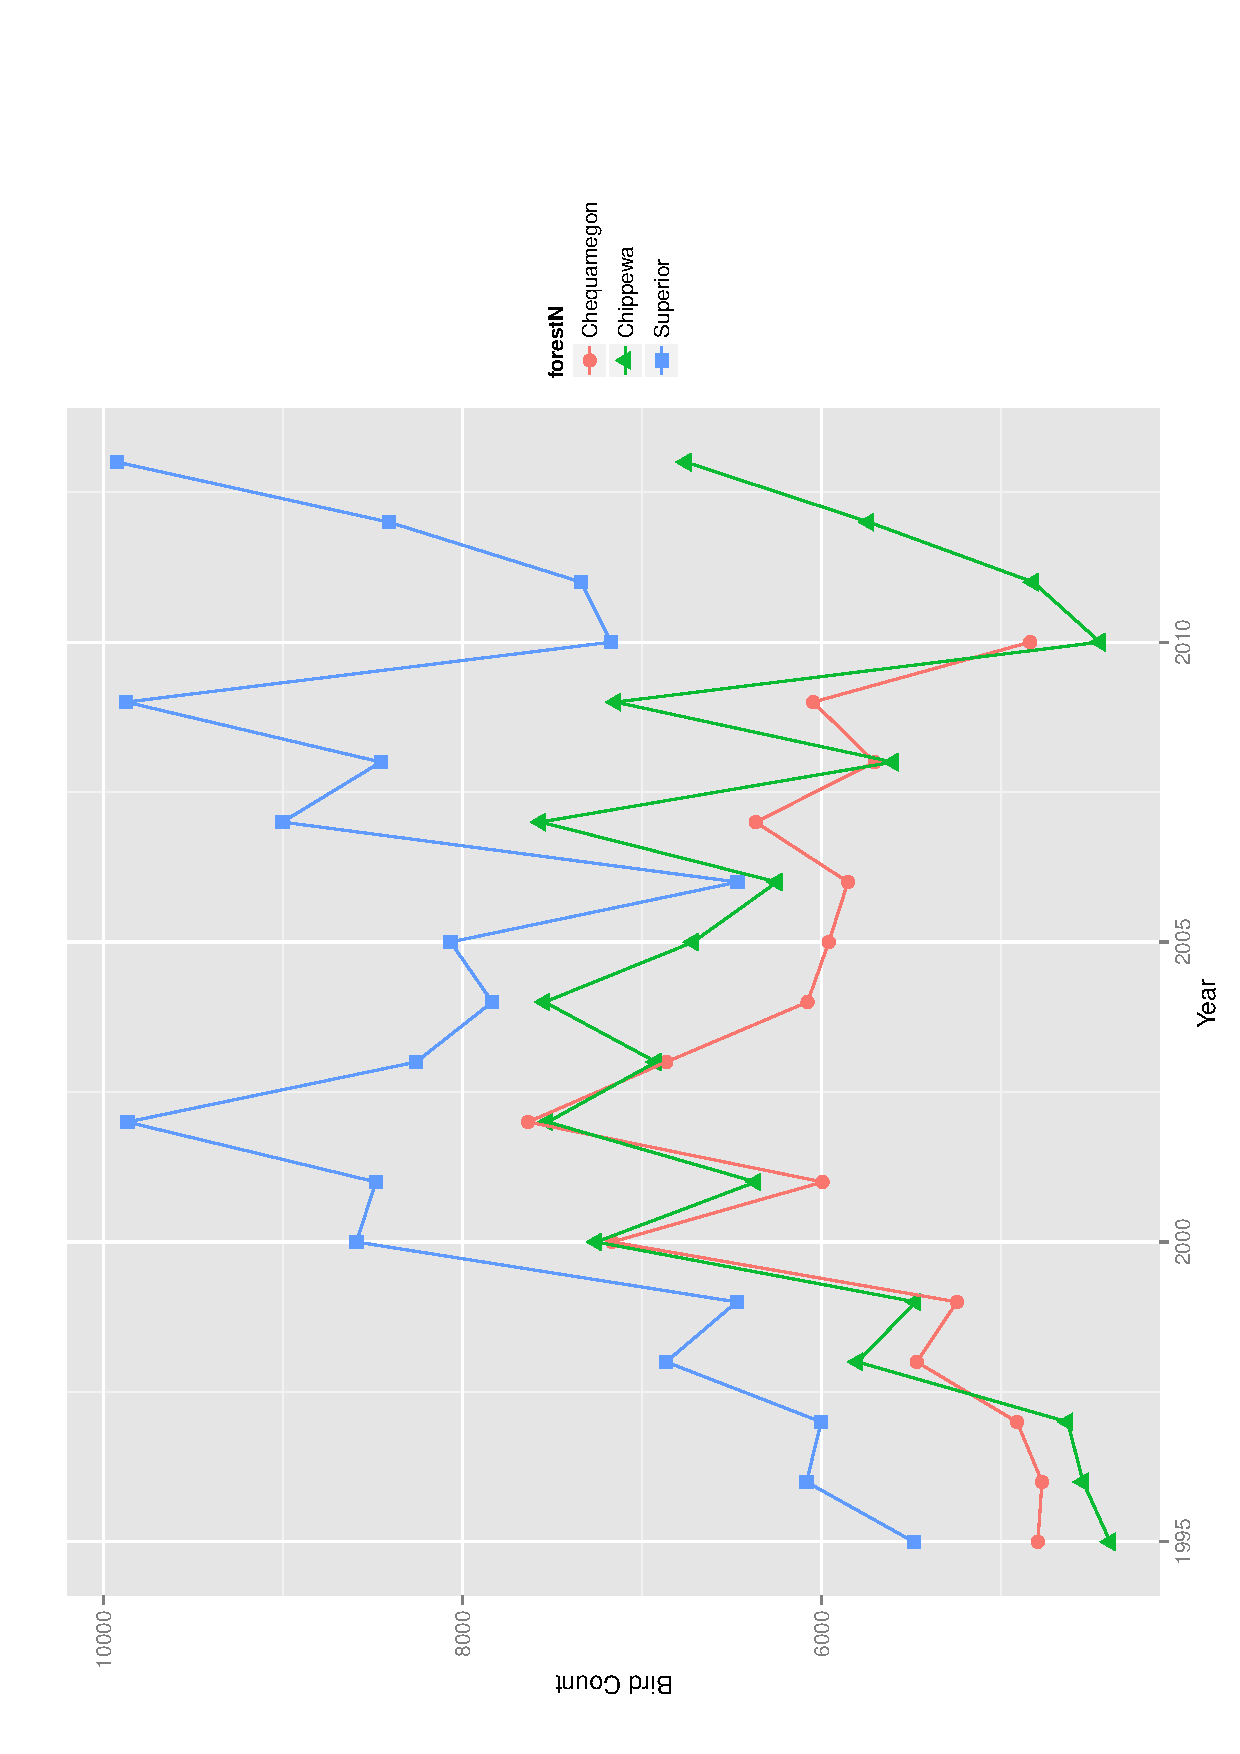
\includegraphics[width =\textwidth]{rawtrend}
 \vspace{-.5in}
\caption{Yearly total birds counts on each forest \label{figtr} }
\end{figure}


We can see Superior is consistently over all years the forest with more bird counts reaching 10000 counts on three time during the monitoring period. The others two forest, Chequamegon and Chippewa show a similar trend in the total bird count. 
 
Overall, it seems to be a first sub-period from 1995 to 2003 where the total bird count is increasing every year but from that this increment stop. From 2003 on Superior forest it seem to oscillate around a little more than 8000 birds while for Chequamegon the count are getting smaller each year. 

% latex table generated in R 3.0.2 by xtable 1.7-1 package
% Tue Apr  1 00:13:08 2014
\begin{table}[ht]
\centering
\caption{Total counts on 2007 for the 10 more abundant species} 
\begin{tabular}{llrrr}
  \hline
Specie & Abbrev & Chequamegon & Chippewa & Superior \\ 
  \hline
Least Flycatcher & OVEN & 1003 & 835 & 1168 \\ 
  Blue Jay & REVI & 823 & 997 & 771 \\ 
  White-throated Sparrow & NAWA & 240 & 348 & 867 \\ 
  Red-eyed Vireo & BLJA & 222 & 199 & 230 \\ 
  Nashville Warbler & CSWA & 211 & 330 & 375 \\ 
  Chestnut-sided Warbler & WTSP & 180 & 387 & 940 \\ 
  Ovenbird & HETH & 175 & 249 & 265 \\ 
  Veery & AMRO & 156 & 102 & 154 \\ 
  Hermit Thrush & LEFL & 155 & 368 & 120 \\ 
  American Robin & VEER &  91 & 402 & 264 \\ 
   \hline
\end{tabular}
\end{table}


There is a big variability of the counts among species. Table \ref{count07} presents the total bird count on year 2007 for the most abundant species, (just to compare it with the on line annual report). We can see that OVEN and REVI are very abundant species among all forest. 

However the structure of abundant is different on each forest. Species like NAWA and WTSP are abundant only in Superior forest, while VEER it is only abundant for Chippewa. In order to model the species count along time it might be better to work separately by forest, we actually restrict the inference to the Superior forest. 

\subsection{ Correlation among Bird Species}

We want to estimate the species correlation over time, we use information only for Superior forest and for the 10 most abundant species in 2007. The idea will be setting up inference on situations similar to the one we have already worked with simulated data. 

The difference "set up" in we will make inference about the correlation among species vary in dimensionality, response variable and covariance matrix prior. In all cases the data will be centered, this might be not realistic but this paper is the covariance matrix and we prefer not considering posibles effects of the mean estimation.  

With ten bird species we have 45 correlation coefficients to estimate, the data model is in every case a normal model with zero mean, $Y \sim N_d(0, \Sigma)$, we estimate each correlation several times, using different contexts. 

\begin{description}
\item[Covariance Prior] The main focus of the paper is to understand the effect of  $\Sigma$ prior distribution. Then we consider all the 4 prior distributions described previously, IW, SIW, HT and SS. 

\item[ Dimensions] The value of $d$ indicate the dimension of the model, we consider two options here. A bivariate case, in which we fit a different model for each pair of species, so this scenario consist in 45 models with 3 parameters each (two variance and the correlation). Also we fit a model for all ten species together, forming one model with 55 parameters (45 correlations and 10 variances). 

\item[Response] We also will use two different response variables. We use the yearly bird count and the yearly average, the latter represent an option with a very little variability in the response while the total count is highly variable. From the simulations results we expect the scale may affect the correlation inference for the IW prior case. 
\end{description}

\begin{figure}[hbpt]
\centering
\includegraphics[width=\textwidth]{rescor}
 \vspace{-.5in}
\caption{Correlation inference results. Posterior median for $\rho$  against Pearson correlation coefficient. 
Columns panel represent the dimension of the model (bivariate or ten-dimensional), row panels represent the response variable (average of the count or total count)  and color of the points represent the covariance prior. \label{fig:coring}  }
\end{figure}

Figure \ref{fig:coring} present the estimated correlations, the posterior median for each model is plotted against the Pearson correlation coefficient. The four panels represent each combination of response and dimension and within each panel there are four estimates for each pair of bird species corresponding to the four priors used. 

These results are quite interesting and match closely with we found on simulated data. When we use the average count as response variable, we see every bayesian is a little bit shrunk towards 0 but the case of the IW this shrinkage is really big. Correlations estimated using IW prior are smaller in absolute value than the rest of the prior options. This effect is expected taking into account that the average count variability is small. 

However results may change if we decide to use a response with high variance as the total count. The IW priors shows a totally different inference picture, now there is no shrunk towards small correlation values and in the case of a ten dimensional model there are several IW correlation median which are actually bigger than Pearson coefficient. 

The SIW, SS and HT priors shows similar behavior no matter which is the response used to estimate the covariance matrix, and estimating correlation with any of these priors will lead to basically same conclusions. Finally if we scale the data to have variance equals to 1 then, IW prior shows a similar behavior than the rest.

\begin{figure}[hbpt]
\centering
\includegraphics[width=\textwidth]{corrmat}
 \vspace{-.5in}
\caption{Correlation matrix among ten species used in the study. Using SS prior, average count, and ten dimensional model \label{fig:mat}}
\end{figure}

Figure \ref{fig:mat} present the estimated correlation matrix using an SS prior, on a ten dimensional model and an average count as a response. There were no negative correlated species among the most abundant ones. We can see there are some species forming a sort of a 'cluster" in the series that all are highly correlated, as  OVEN, REVI and CSWA (maybe WTSP could be in this group too). 

On the other hand there are a couple of species which shows small correlations with all the rest, this is specially true for LEFL and also AMRO.   We plot the trend of these five species in the next figure. 

\begin{figure}[hbpt]
\centering
\includegraphics[width=\textwidth]{spcor}
 \vspace{-.5in}
\caption{Trend in some selected species. OVEN, REVI and CSWA are highly correlated while LEFL and AMRO shows no correlation with other species. \label{trend}}
\end{figure}

Figure \ref{trend}  shows the dynamics for the five species identify on the correlation matrix. AS the data are centered, the lines represent the difference between the average yearly count and the historical mean for that species. The three species with high correlation shows the same temporal pattern, a sort of inverted u-shape specially marked on the case of OVEN. The two species with small correlation have a very stable pattern with no big departures from its own mean. 

\section{Discussion} 

We compare several choices for covariance matrix prior, this comparison is based on simulation and visualization tools since there is typically no analytical results to compare them. 

At a first step, locking at simulations from the prior we see that IW constraint the covariance matrix parameter implying strong dependence among these individual matrix components, correlations tend to be small when variances are small and also the variances from different components are positive correlated.  Priors SIW and HT shows similar characteristics than IW but both seem to be more flexible than IW prior. The case of SS is the one presenting the most flexibility since variances and correlations are by construction independent.

In practice what determines the inference for the bayesian model is not the prior but how the posterior looks like. Posterior simulation results for IW prior show this options maintain the problems we see already in the prior.  The correlation estimate is affected by the scaling of the data, when the variance is low the posterior mean is shrunk towards 0 regardless the true value of the correlation coefficient. 

The other three options for $\Sigma$ prior does not show evident problems capturing the true correlation values for this simulation exercise. Even  SIW and HT who show similar prior characteristic than IW, its flexibility is enough to ensure good results estimating correlations. As we expected SS prior show no big problems estimating  covariance. 

The main question that arise at this point is What prior should we use ? 

From a modeler point of view, the SS prior flexibility is appealing since we can model correlations and variance in separate fashion and will be the data what define its relationship. 
We implement SS strategy using a lognormal prior for standard deviations because this was the original prooposed by \cite{barnard2000}, but we could use any other prior, for instance a half-t or uniform which are better within the hierarchical models context.  In the scaled inverse Wishart prior, the variance parameters are compose by the product of an inverse gamma times the scales parameters which here have been set up as lognormals but it could be done differently, however it always be a partial solution compare to the SS one. 

From a computational perspective we expect the SS prior the most complex, since all the others conserve the conjugacy properties of the inverse Wishart distribution This is specially relevant for a Gibbs sampler, where conjugacy allow to get a full Gibbs step instead a metropolis one, Using STAN software which is base in Hamiltonian Monte Carlo strategy to obtain samples from posterior there is no that much cost to paid for using a non conjugate prior as the SS.  Results for SIW prior show much better computational performance than the rest with the best time samples ratio among all choices.  

In summary, the answer to the previous question may depend on which are the computational resources we are working with 

\begin{itemize}
\item  if it is posible to use a HMC sampler as STAN the separation strategy proposed by \cite{banard2000} gives modeling flexibility and good inferences properties. But computational performance is poor, this should be improve in order to use this strategy as the general default option. Probably sampling directly from the correlation matrix distribution is the way to do this. 

\item Whenever we use Gibbs base samplers (as JAGS or BUGS) a prior which maintain conjugacy might be preferable such as the scaled inverse Wishart. This prior shown good computational performance and nice inference properties.  

\item For some models the samplers does not allow to fit these priors and we are constraint to use the classical inverse Wishart distribution, in this case, we may recommend to scale the data first in order to avoid possible biased estimates for correlations. 
\end{itemize}

The problem of setting covariance priors is fairly complex and the simulation exercise presented here is far from deal with it in all its complexity. So there are multiple ways in which we could continue with this line of work. However, there are two that seems the more natural way to go. A first next step would be to extend this study into the context to hierarchical models where the covariance matrix prior is not for the data model but for modeling a set of coefficient in a linear predictor. Secondly, a deeper study on priors for correlation matrices as the LKJ prior could give better ways to implement the separation strategy. 

\bibliographystyle{asa}      
\bibliography{report_year}      


\end{document}
%============================================================================================
%% 	LINEAR MODEL STUFF MOVE OUT OF THE REPORT 


%\subsection{Hierarchical Linear Models}

%Usually the multivariate normal distribution does not appear directly to model data, the common models assumes independence along observations and when this assumption it is not present the covariance matrix is modeled with a specific structure such as compound cemetery in a random effects model. 

%Instead multivariate normal model is a very commonly used as a distribution of a linear model coefficients within the context of a hierarchical model. Le asume we are interested in a model like  $Y_s \sim N(X_s\beta_s, \sigma_s)$ where the subscript $s$ is representing the different groups in the model. 
%In the concrete data set, we use time as the main covariate variable and a response variable changing over time, also the data are grouped according bird, then $Y_{ts}$ will be related to the average bird count for group $s$ at time $t$ and an model example could be $Y_ts \sim N(\beta_{1s} + t\beta_{2s}, \sigma_s)$. 

%In order to make inference from this modle within a bayesian framework, we need to decide priors for $(\beta_s, \sigma_s)$ parameters. One key decision for this choice is how to combine information across groups. We may want to set a separate prior for each parameter within each group, making each group model completely independent from the rest. On the opposite side we could combine all the groups into one set of parameters $(\beta_s, \sigma_s) = (\beta, \sigma)$. Finally as a compromise between the previous options we can allows different parameters for each group but all with common prior distribution, i.e. a hierarchical model. 
%
%These options on how combine information across groups can be done independently for $\beta_s$ and $\sigma_s$, which lead us to a nine ways setting up the prior distributions for all the parameters in the model. Table \ref{stmod} presents the basic choices of models we just described, rows of the table are the three ways we can combine the groups information for the $\beta_s$ coefficients and the columns represents the same thing but for $\sigma_s$ instead. The result are nine models, each of the nine cells in Table \ref{stmod} represents one of those combination. 
% 
%\begin{table}[h]
%\caption{Basic Prior Structure Choices. In all cases the data model consist in a multivariate regression $Y_s \sim N(X_s\beta_s,\sigma_s^2)$, also in all models the prior for the vector $\beta_s$ is a normal distribution, $N(\mu, \Sigma)$ but  parameters $\mu$ and $\Sigma$ might be learned from the data or set as a fixed value. \label{stmod} } 
%\begin{tabular}{|l|ccc|} \hline \hline
%& Same $\sigma$s ($\sigma_s=\sigma$) & Hierarchical $\sigma$s & Different $\sigma$s \\ \hline\hline
%Same   
%%&$Y_s \sim N(X_s\beta,\sigma^2)$&$Y_s \sim N(X_s\beta,\sigma_s^2)$& $Y_s \sim N(X_s\beta, \sigma_s^2)$ \\
%$\beta$s &$\mu=\mu_0, \Sigma=\Sigma_0$ &$\mu=\mu_0, \Sigma=\Sigma_0$&$\mu=\mu_0, \Sigma=\Sigma_0$ \\
%($\beta_s = \beta$ ) & $\sigma\sim unif(0, v_0)$ &$\sigma^2_s\sim IG(\alpha_s/2, \alpha_s\lambda_s/2)$& $\sigma_s\sim unif(0, v_0)$ \\ 
%& & $\alpha_s \sim unif(0,a_0)$ & \\ 
%& & $\lambda_s\sim unif(0,l_0)$ & \\ \hline 
%hierarchical $\beta$s
%%&$Y_s \sim N(X_s\beta,\sigma^2)$&$Y_s \sim N(X_s\beta,\sigma_s^2)$& $Y_s \sim N(X_s\beta, \sigma_s^2)$ \\
%%&$\beta_s\sim N(\mu, \Sigma)$&$\beta_s\sim N(\mu, \Sigma)$ & $\beta_s\sim N(\mu,\Sigma)$ \\
%& $\mu \sim N(\psi_0, \Psi_0) $ & $\mu \sim N(\psi_0, \Psi_0) $ & $\mu \sim N(\psi_0, \Psi_0) $ \\ 
%& $\Sigma \sim IW(R_0,d_0)$& $\Sigma \sim IW(R_0,d_0)$& $\Sigma \sim IW(R_0,d_0)$ \\  
%&$\sigma\sim unif(0, v_0)$ &$\sigma^2_s\sim IG(\alpha_s/2, \alpha_s\lambda_s/2)$& $\sigma_s\sim unif(0, v_0)$ \\ 
%& & $\alpha_s \sim unif(0,a_0)$& \\
%& & $\lambda_s\sim unif(0,l_0)$ & \\ \hline 
%different $\beta$s
%%&$Y_s \sim N(X_s\beta,\sigma^2)$&$Y_s \sim N(X_s\beta,\sigma_s^2)$& $Y_s \sim N(X_s\beta, \sigma_s^2)$ \\
%%&$\beta_s\sim N(\mu_0, \Sigma_0)$&$\beta_s\sim N(\mu_0, \Sigma_0)$&$\beta_s\sim N(\mu_0, \Sigma_0)$ \\
%&$\mu=\mu_0, \Sigma=\Sigma_0$ &$\mu=\mu_0, \Sigma=\Sigma_0$&$\mu=\mu_0, \Sigma=\Sigma_0$ \\
%&$\sigma\sim unif(0, v_0)$ &$\sigma^2_s\sim IG(\alpha_s/2, \alpha_s\lambda_s/2)$& $\sigma_s\sim unif(0, v_0)$ \\ 
%& & $\alpha_s \sim unif(0,a_0)$ & \\
%& & $\lambda_s\sim unif(0,l_0)$ & \\ \hline\hline
%\end{tabular} \\
%\tiny{Every letter with subscript 0 represent a numeric value and is not learned from data, $IW$ represents an inverse Wishart distribution and $IG$ an inverse gamma distribution.}
%\end{table}
%
%Some comments about the models and notation contain in Table \ref{stmod}. 
%First, all the symbols with ''0'' subscript represent numerical known values not parameters we learn from data. Usually these parameter are set to assure the non informativity of the prior. For instance $v_0$, $a_0$ and $l_0$ are the upper limits of uniforms distributions for variance parameter or hyperparameter and then will be set as very high numerical values. 
%
%Second, every model is written in matrix form. Vector $Y_s$ represent all observations for group $s$, $Y_s =  (Y_{s1},Y_{s2},\dots,Y_{sn})^{'}$, in same way $X_s$ is a $n \times k$ matrix containing the observed values for $k$ predictor variables. 
%Accordingly, parameters are also in matrix form, so $\beta_s$ and $\mu$ are $k$-dimensional vectors representing each predictor effect for the group $s$ and its prior mean, while $\Sigma$ is the $k\times k$ covariance matrix for $\beta_s$ (note that $\mu_0$ and $\Sigma_0$ are numerical values not parameters, so they are not vector or matrices just scalar known values). 
%
%Third, in every case the deepest layer in the model is some uniform distribution for a variance parameter or for a variance hyper-parameter. We choose a uniform prior on standard deviation scale for $\sigma_s$ and its related hyperparameters, this is following Gelman recommendation on REF, but we could set a different options as inverse gamma flat prior as recomended on REF or an improper prior. 
%
%As examples, we describe the three models that lies in the diagonal of the table \ref{stmod}. 
%
%The first model consist in a situation where we are ignoring the existence of different group and just estimating one set of $\beta$ and one value of $\sigma$ so this is actually one regression on the entire data. On the other hand, the ''last'' cell in the table (column 3, row 3) is representing a separate regressions for each group with flat priors on all parameters. In this case the $\Sigma_0$ matrix is a diagonal matrix
%
%Finally, the central cell model represent a fully hierarchical model in both $\sigma$ and $\beta$. The covariance matrix $\Sigma$ is learned form data, so we want to model the dependency across the linear predictor coefficient.  Here the choice of $p(\Sigma)$ is really important, ''it determines the nature of the shrinkage of the posterior of the individual $\beta_j$ towards a common target'' (\cite{barnard2000}). 
%What is the effect of the covariance matrix prior on the inference about the linear model coefficients ?  This is an important question we would like to address. 



%\subsection{ Bird Populations trends} 
%According to (REF, Etterson) one of the basic research goals in Ecology consist on understand the distribution and abundance of the animal population. In this work, the particular goal will be to explore alternatives to model the time trends in Western Great Lakes Birds population over 1994 to 2011. As a starting point we consider separate regression equations for each specie and forest, a model for one species is represented on equation \ref{mod1}. 
%\begin{eqnarray}
%\nonumber Y_{ts} &=&  \beta_{0s} + \beta_{1s}t + \beta_{2s}t^2 + \epsilon_{ts}  \\
%\epsilon_{ts} &\sim& N(0,\sigma_{s}^2)
%\label{mod1}
%\end{eqnarray}
%where $Y_{ts}$ represent the average bird count on year $t$ in the forest $f$ for the specie $s$. From a bayesian point of view this consist in a hierarchical Normal model where $Y_{ts}\vert (\beta_{0s},\beta_{1s},\beta_{2s},\sigma_{s}) \sim N(\beta_{0s}+\beta_{1s}t+\beta_{2s}t^2, \sigma_{s})$ and all parameters are independents with flat priors and different values for each species. 
%
%There are 73 species and we fit the model \ref{mod1} for 3 different forests there are 219 individual species regression models in total. In addition, we consider two variants from \ref{mod1}. First, it is not clear that we need to include a quadratic term in the regression term so we may consider a simple regresion only. Second, it is common to log transform the average counts. So, for each species we consider 4 models including two types of response variable (in logs and average count) and two set of predictors (quadratic and only linear). 
% 
%Along this report the parameters of interest will be the regression slope for each species.  Figure \ref{histm1} presents these slopes median for each species on every scenario we run for all three forest. There are 12 panels, each row represent one forest (Chequamegon, Chippewa and Superior) and each column represent one type of model (linear in logs, quadratic in logs, linear with counts and quadratic with counts).  
%\begin{figure}[h!]
%\centering
%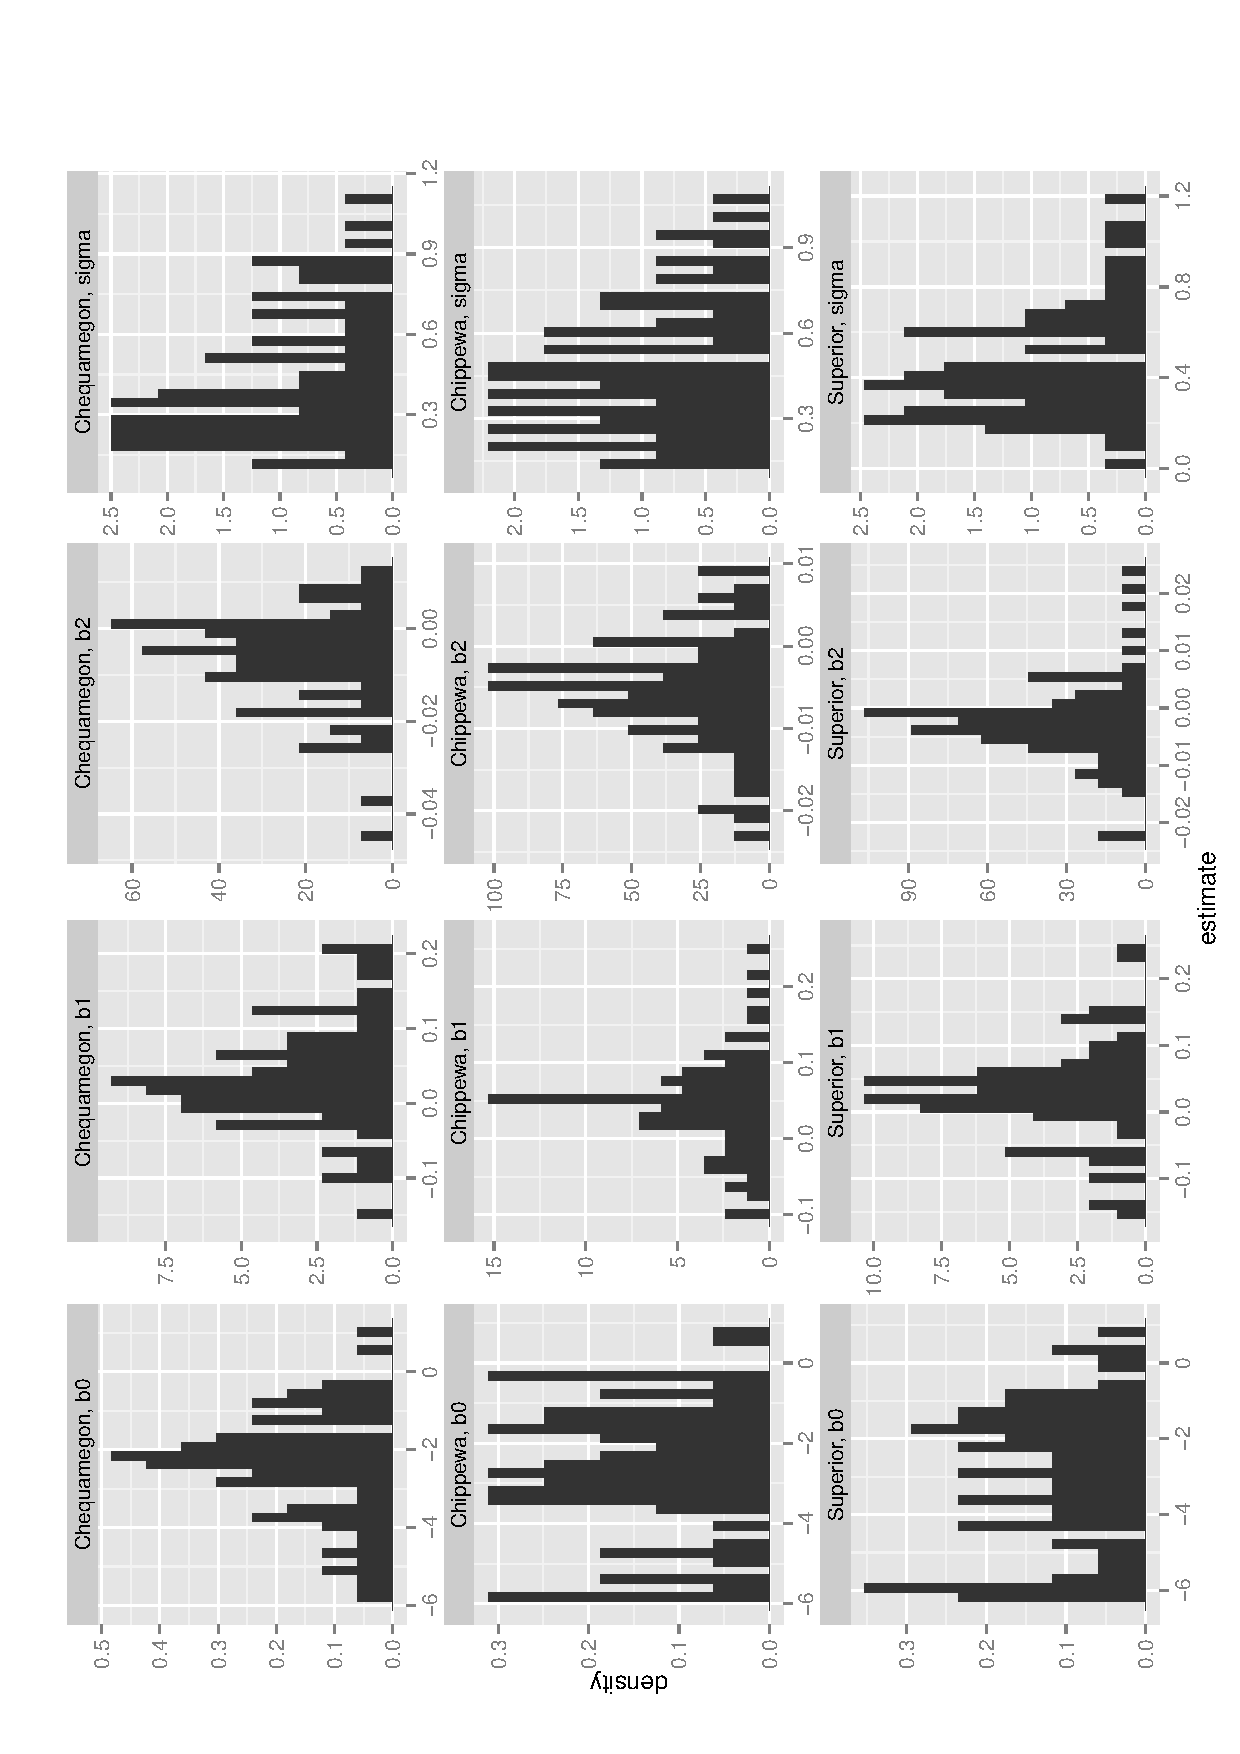
\includegraphics[scale=.5]{hist_m1}
%\caption{Species slopes from model \ref{mod1} . \label{histm1}}
%\end{figure}
%
%The slopes histograms are similar on the 3 forest within each model type. The model with the log transformed response seem to present a more symmetric distribution of the slopes, when we use the average counts most of the slopes are very close to zero value except for a few species with high slope values. 
%
%Next, we explore the bivariate relation among the coefficients within each regression. With this in mind we can see a scatter matrix of the estimated coefficients in Figure \ref{pairss1}. The main point to see here is a negative relation between the slope and the quadratic term for all forest, is .67, .82 and .83 on Chequamegon, Chippewa and Superior respectively. (KAISER Dix it: while polynomials are wonderfully flexible functions for describing data patterns, they do not lend themselves to interpretation of coefficient values -different combinations of constant, linear, and quadratic terms can lead to quite similar functions over a finite range of covariate values) 
%
%\begin{figure}[h!]
%\centering
%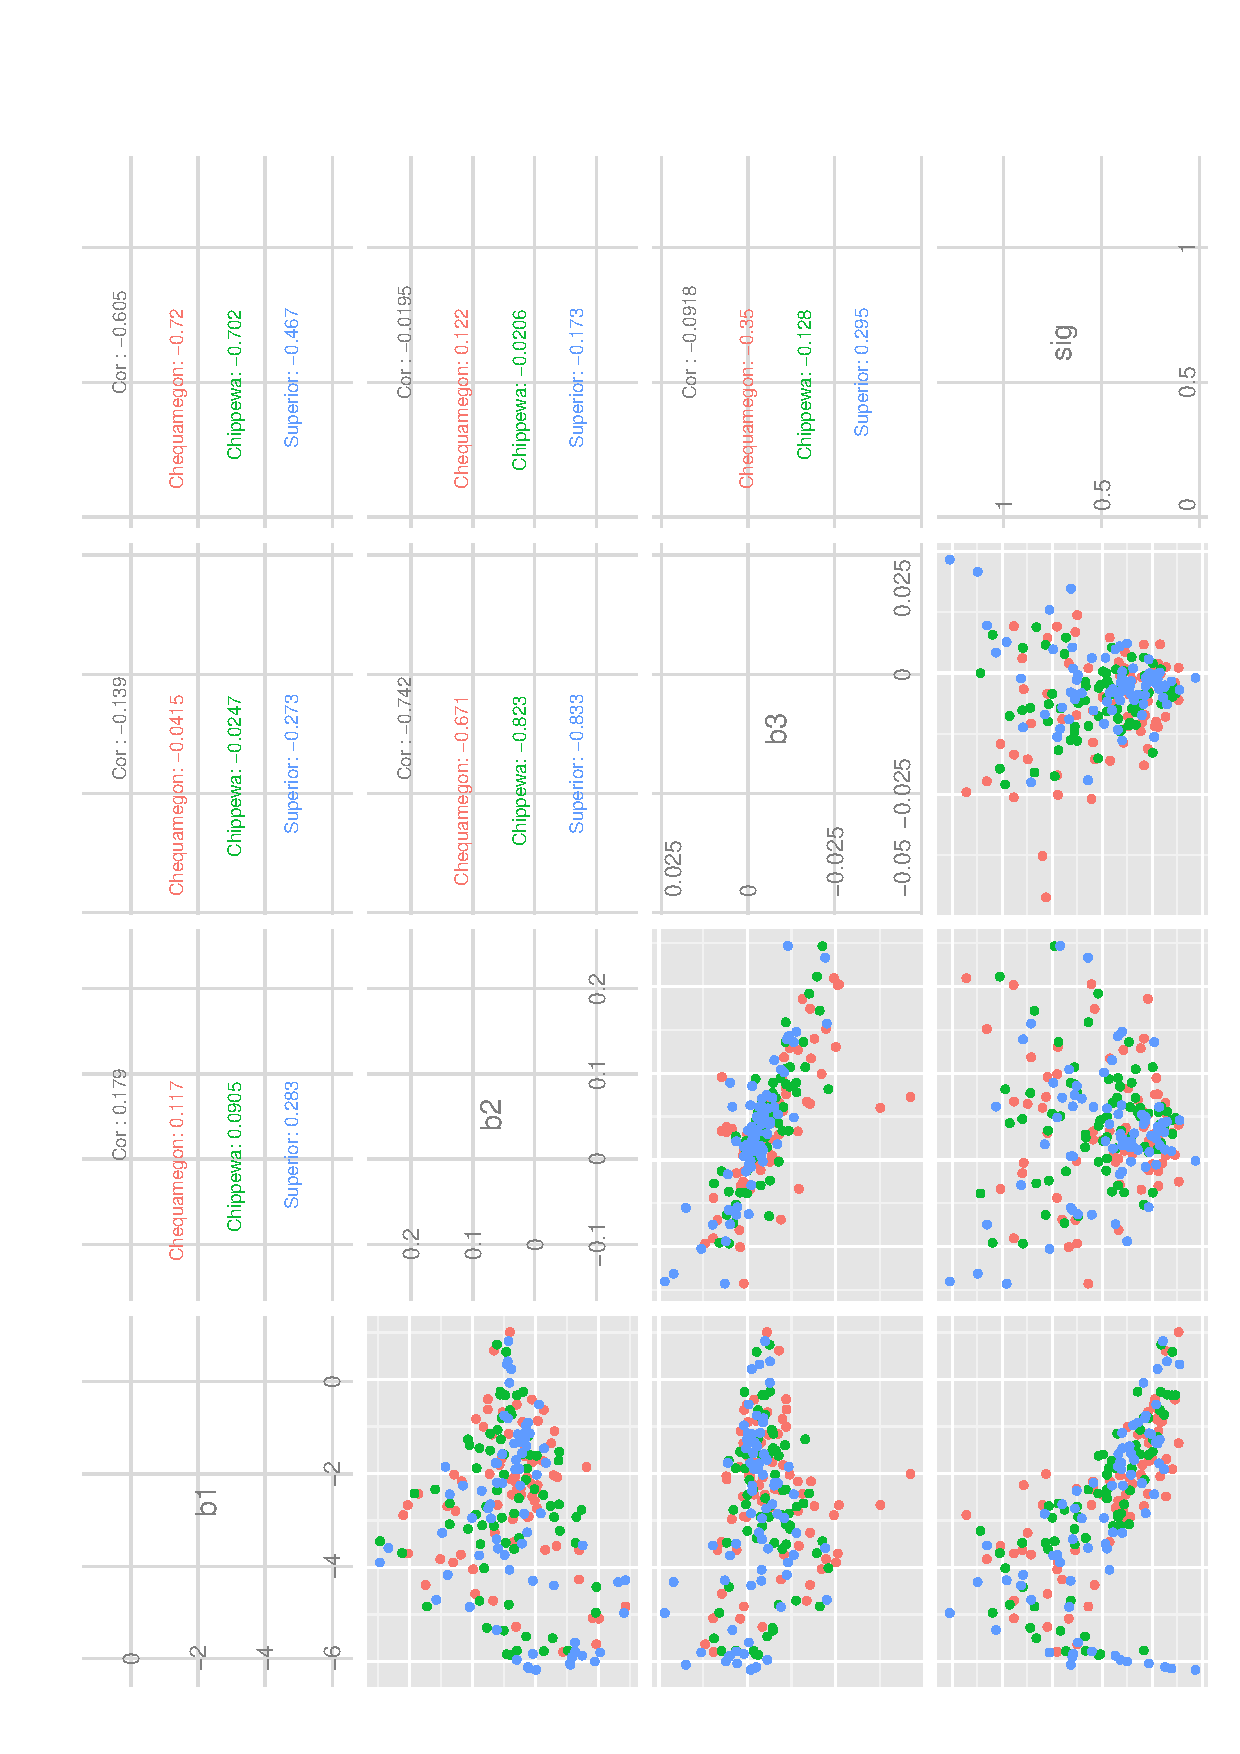
\includegraphics[scale=.6]{scat_m1}
%\caption{Bivariate relation among coefficients of model \ref{mod1}. \label{pairs1}}
%\end{figure}
%Also, there is a negative relation between between intercept and variance, specially for Chequamegon and Chippewa forest. Maybe the main message for this plot is that we should not treat this parameters as independent and try to include their dependence into the model we are fitting. 
%\begin{figure}[h!]
%\centering
%\includegraphics[height=12cm, width=5cm, angle=-90]{gelman.ps}
%\caption{Multivariate Gelman Diag statistic for all models. \label{gel1}}
%\end{figure}
%
%\begin{figure}[h!]
%\centering
%\includegraphics[scale=.6, angle=-90]{slp_bet.ps}
%\caption{ Slope estimates within each type of variance model}
%\end{figure} 
%
%\begin{figure}[h!]
%\centering
%\includegraphics[scale=.6, angle=-90]{rates.ps}
%\caption{ Change Rates within each type of variance model}
%\end{figure} 
%
%\begin{figure}[h!]
%\centering
%\includegraphics[scale=.6, angle=-90]{var_hhll.ps}
%\caption{$Sigma$ posterior distribution visualization plot}
%\end{figure} 
%
%\begin{figure}[h!]
%\centering
%\includegraphics[scale=.6, angle=-90]{var_hhql.ps}
%\caption{$Sigma$ posterior distribution visualization plot}
%\end{figure} 
%%%%%%%%%%%%%%%%%%%%%%%%%%%%%%%%%%%%%%%%%%%%%%%%%%%%%%%%%%%%%%%%%%%%%%%%
